\documentclass[a4paper,12pt]{article}

\usepackage{amsfonts, amsmath, amssymb, amsthm, enumitem, fancyhdr, graphicx}
\usepackage[margin=3.5cm]{geometry}
\allowdisplaybreaks
\pagestyle{fancy}
\rhead{Erick Lin}

\renewcommand{\thesubsection}{\arabic{subsection}}
\newtheorem{theorem}{Theorem}
\newtheorem{lemma}[theorem]{Lemma}

\begin{document}

\section*{MATH 4431 -- HW5 Solutions}
\begin{enumerate}
    \item[1.]
        \boldmath\textbf{For each $i$, let $X_i = \{0, 1\}$ be the two-point set with the discrete topology. Show that $\prod_{i = 1}^\infty X_i$ is a Cantor set.
        }\unboldmath \par
        %By Theorem IV.5, $\prod_{i = 1}^\infty X_i$ is the Cantor set if and only if it is a perfect, totally disconnected, compact metric space, so we show each of these properties as follows.
        A point in $\prod_{i = 1}^\infty X_i$ is a countably infinite binary sequence $\{ a_i \}_{i = 1}^\infty$. Then the map from the sequence onto the real number
        \begin{align*}
            \sum_{i = 1}^\infty \frac{2a_i}{3^i}
        \end{align*}
        maps onto the standard Cantor set $C$ since each $n \geq 1$, the partial sum $\sum_{i = 1}^n \frac{2a_i}{3_i}$ maps into the set $A_n$ given in the definition of $C$, which can be proved by induction. \par
        The map is also a bijection since it determines the inverse of a point in $C$ as, for each $i$,
        \begin{align*}
            a_i = \begin{cases}
                0 \text{ if the point lies in the leftmost third} \\
                1 \text{ if the point lies in the rightmost third}
            \end{cases},
        \end{align*}
        of the current interval, if the current interval is initially $[0, 1]$ and inductively defined as the same third in which the point lies. \par
        Furthermore, the inverse map is continuous because the projection map onto each component $a_i$ is continuous, being constant on some closed and open neighborhood containing that point. \par
        We also know that $C$ is compact, that each $X_i$ is trivially Hausdorff due to the discrete topology, and that countable products of Hausdorff spaces are Hausdorff. Therefore, the inverse map is a continuous bijection from a compact space to a Hausdorff space, and so it is a homeomorphism. Being homeomorphic to a Cantor set, $\prod_{i = 1}^\infty X_i$ is also a Cantor set.

    \item[7.]
        \boldmath\textbf{Let $p$ and $q$ be two points in the Cantor set $C$. Show that there is a homeomorphism $h : C \to C$ such that $h(p) = q$.
        }\unboldmath \par
        From Problem 1, we know that $C$ is homeomorphic to the space of infinite binary sequences, so we can let $\{p_i\}_{i = 1}^\infty$ and $\{q_i\}_{i = 1}^\infty$ respectively be the points corresponding to $p$ and $q$ in the latter space. Showing that there is a homeomorphism that maps $\{p_i\}_{i = 1}^\infty$ to $\{q_i\}_{i = 1}^\infty$ in this space implies that there is also one that maps $p$ to $q$ in $C$, since the homeomorphism relation is an equivalence relation. \par
        Now for each $i \geq 1$, if we define $f_i : \{0, 1\} \to \{0, 1\}$ by
        \begin{align*}
            f_i(x) = \begin{cases}
                x, &p_i = q_i \\
                1 - x, &p_i \neq q_i
            \end{cases}.
        \end{align*}
        It is easy to see that each $f_i$ is bijective. Each $f_i$ is also continuous with continuous inverse since every subset of $\{0, 1\}$ is open and closed under the discrete topology, so $f_i$ is a homeomorphism.
        \begin{lemma} \label{lem:prod-homeo}
            Any countable product of homeomorphisms is a homeomorphism.
        \end{lemma}
        \begin{proof}
            We show this for any product of two homomorphisms, which easily extends to any countable number by induction. It is clear that a product of two bijections is a bijection, and we also know that the product of two continuous maps is continuous. Finally, if each component function has a continuous inverse, then any open set in the domain maps to an open set in each of the functions, and the product of these two resulting open sets is a basic open set under the product topology. Thus, the product also has continuous inverse.
        \end{proof}
        By Lemma \ref{lem:prod-homeo}, $f = \prod_{i = 1}^\infty f_i$ is a homeomorphism, and by construction, $f(\{p_i\}_{i = 1}^\infty) = \{q_i\}_{i = 1}^\infty$. \par

    \item[10.]
        \boldmath\textbf{Let $D$ be a disk and $I$ be an interval in $\partial D$. If $\Sigma$ is a surface and $f : I \to \partial \Sigma$ is an embedding, then show that the surface
            \begin{align*}
                \Sigma \cup_f D
            \end{align*}
            is homeomorphic to $\Sigma$.
        }\unboldmath \par
        Since $I$ is connected, $f(I)$ is also, so if we denote $B$ as the connected component of $\partial \Sigma$ containing $f(I)$, then there is an open set $U \subset \Sigma$ containing $B$ that is homeomorphic to $S^1 \times [0, 1)$, which we know is equivalent $S^1 \times [-1, 0]$, but this means $U$ is closed and compact as well, being a finite product of closed and compact sets. Being a closed subset of a compact space, $B$ must be compact as well. Thus, by Lemma V.7, $B \cong \{0\} \times S^1 \cong S^1$ (projection to the second component is a homeomorphism because any projection and its inverse, an inclusion map, are continuous, and also bijective because the first component has only one possible value).
        \begin{lemma}
            The space obtained from two disks by gluing them along intervals in their boundary is homeomorphic to a disk.
        \end{lemma}
        \begin{proof}
            If $D_1$ and $D_2$ are disks with $I_1$ and $I_2$ being intervals along $\partial D_1$ and $\partial D_2$ respectively, then using the fact that closed intervals are homeomorphic to one another and so are open intervals, we can determine an identification map $f : D_1 \cup D_2 \to D$ piecewise, where $D$ is the unit disk centered at the origin, by
            \begin{itemize}
                \item 
                    letting $f : I_1 \to \{0\} \times [-1, 1]$ be an arbitrary homeomorphism,
                \item
                    defining $f : I_2 \to \{0\} \times [-1, 1]$ by $f(p) = f(h(p))$ where $h : I_1 \to I_2$ is an arbitrary homeomorphism,
                \item
                    letting $f : \partial D_1 \setminus I_1 \to \{ (x, y) \in \partial D_1 : x < 0 \}$ be an arbitrary homeomorphism,
                \item
                    letting $f : \partial D_2 \setminus I_2 \to \{ (x, y) \in \partial D_2 : x > 0 \}$ be an arbitrary homeomorphism, and
                \item
                    extending $f$ to a homeomorphism from each newly constructed boundary component to its respective interior.
            \end{itemize}
            $D$ is thus the identification space.
        \end{proof}
        Therefore, $B \cup_f D \cong D$, so gluing $D$ to $\Sigma$ using $f$ preserves $\Sigma$ up to homeomorphism.

    \item[11.]
        \boldmath\textbf{Show that for any connected surface $\Sigma$ and points $p$ and $q$ in $\Sigma$, there is a homeomorphism $h : \Sigma \to \Sigma$ such that $h(p) = q$.
        }\unboldmath \par
        From Problem 9, we can see that there is always an embedding $e : D^2 \to \Sigma$ such that $p$ and $q$ are contained in the interior of the image of $e$, even if $p$ and $q$ are in an open set homeomorphic to $\mathbb{R}^2$, and since $\Sigma \cong \mathbb{R}^2$, it only remains to show that there is a homeomorphism $h : D^2 \to D^2$ such that $h(p) = q$ and the boundary of $D^2$ is fixed. \par
        Considering $D^2$ in the complex plane, if we define the homeomorphism
        \begin{gather*}
            f_1(z) = \frac{z - p}{1 - \overline{p} z} \\
            f_2(z) = \frac{z - t f(q)}{1 - t\overline{f(q)} z},
        \end{gather*}
        then $f_2 \circ f_1(p) = -f_2 \circ f_1(p)$. Now, the homeomorphism
        \begin{align*}
            h(z) = ze^{i(1 - |z|)\pi/(1 - |f_2 \circ f_1(p)|)}
        \end{align*}
        interchanges $f_2 \circ f_1(p)$ and $f_2 \circ f_1(q)$ and fixes the boundary of $D^2$. Therefore, the homeomorphism $f_1^{-1} \circ f_2^{-1} \circ h \circ f_2 \circ f_1$ interchanges $p$ and $q$, and in particular sends $p$ to $q$, while fixing the boundary.

    \item[14.]
        \boldmath\textbf{What surface in our classification is $N_{1, 1} \# \Sigma_{2, 2}$ homeomorphic to?
        }\unboldmath \par
        This surface has three boundary components, because $N_{1, 1}$ is $N_1$ with one disk removed and $\Sigma_{2, 2}$ is $\Sigma_2$ with two disks removed. Since removing a $2$-handle decreases the Euler characteristic by $1$,
        \begin{align*}
            \chi(N_{1, 1} \# \Sigma_{2, 2}) &= \chi(N_{1, 1}) + \chi(\Sigma_{2, 2}) - 2 \\
            &= \chi(N_1) + \chi(\Sigma_2) - 5 \\
            &= (2 - 1) + (2 - 2 \cdot 2) - 5 \\
            &= -6.
        \end{align*}
        The surface is non-orientable and thus homeomorphic to $N_{n, 3}$ for some $n \geq 1$, and solving for $n$,
        \begin{align*}
            -6 = \chi(N_{n, 3}) = 2 - n - 3 \Rightarrow n = 5
        \end{align*}
        so $N_{1, 1} \# \Sigma_{2, 2} \cong N_{5, 3}$ where $\cong$ represents the homeomorphism relation with respect to surfaces.

    \item[15.]
        \boldmath\textbf{Identify the surfaces in the figures below.
        }\unboldmath \par
        \begin{center}
            
\includegraphics[scale=0.8]{hw5_fig1}
            \qquad \qquad
            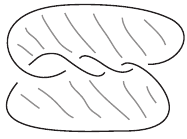
\includegraphics[scale=0.8]{hw5_fig2}
        \end{center}
        By tracing along the boundary, we can see that the surface $S_1$ in the first figure has one boundary component. Furthermore, it is non-orientable since it has only one side, so overall $S_1 \cong N_{n, 1}$ for some $n \geq 1$. Lastly, the surface decomposes into a set of three $0$-handles and three $1$-handles, which means that $\chi(S_1) = 3 - 3 + 0 = 0$. Solving for $n$, we have
        \begin{align*}
            0 = \chi(N{n, 1}) = 2 - n - 1 \Rightarrow n = 1
        \end{align*}
        and thus $S_1 \cong N_{1, 1}$. \par
        The surface $S_2$ in the second figure has two boundary components, is orientable because it has two sides and hence homeomorphic to $\Sigma_{n, 2}$ for some $n \geq 1$, and decomposes into a set of two $0$-handles and four $1$-handles so $\chi(S_2) = 2 - 4 + 0 = -2$. Solving for $n$, we have
        \begin{align*}
            -2 = \chi(\Sigma_{n, 2}) = 2 - 2n - 2 = -2n \Rightarrow n = 1
        \end{align*}
        and thus $S_2 \cong \Sigma_{1, 2}$.
\end{enumerate}

\end{document}
